% Options for packages loaded elsewhere
\PassOptionsToPackage{unicode}{hyperref}
\PassOptionsToPackage{hyphens}{url}
\PassOptionsToPackage{dvipsnames,svgnames,x11names}{xcolor}
%
\documentclass[
  11pt,
  letterpaper,
  DIV=11,
  numbers=noendperiod]{scrartcl}

\usepackage{amsmath,amssymb}
\usepackage{lmodern}
\usepackage{iftex}
\ifPDFTeX
  \usepackage[T1]{fontenc}
  \usepackage[utf8]{inputenc}
  \usepackage{textcomp} % provide euro and other symbols
\else % if luatex or xetex
  \usepackage{unicode-math}
  \defaultfontfeatures{Scale=MatchLowercase}
  \defaultfontfeatures[\rmfamily]{Ligatures=TeX,Scale=1}
\fi
% Use upquote if available, for straight quotes in verbatim environments
\IfFileExists{upquote.sty}{\usepackage{upquote}}{}
\IfFileExists{microtype.sty}{% use microtype if available
  \usepackage[]{microtype}
  \UseMicrotypeSet[protrusion]{basicmath} % disable protrusion for tt fonts
}{}
\makeatletter
\@ifundefined{KOMAClassName}{% if non-KOMA class
  \IfFileExists{parskip.sty}{%
    \usepackage{parskip}
  }{% else
    \setlength{\parindent}{0pt}
    \setlength{\parskip}{6pt plus 2pt minus 1pt}}
}{% if KOMA class
  \KOMAoptions{parskip=half}}
\makeatother
\usepackage{xcolor}
\usepackage[margin=2.4cm, footskip=1cm]{geometry}
\setlength{\emergencystretch}{3em} % prevent overfull lines
\setcounter{secnumdepth}{-\maxdimen} % remove section numbering
% Make \paragraph and \subparagraph free-standing
\ifx\paragraph\undefined\else
  \let\oldparagraph\paragraph
  \renewcommand{\paragraph}[1]{\oldparagraph{#1}\mbox{}}
\fi
\ifx\subparagraph\undefined\else
  \let\oldsubparagraph\subparagraph
  \renewcommand{\subparagraph}[1]{\oldsubparagraph{#1}\mbox{}}
\fi


\providecommand{\tightlist}{%
  \setlength{\itemsep}{0pt}\setlength{\parskip}{0pt}}\usepackage{longtable,booktabs,array}
\usepackage{calc} % for calculating minipage widths
% Correct order of tables after \paragraph or \subparagraph
\usepackage{etoolbox}
\makeatletter
\patchcmd\longtable{\par}{\if@noskipsec\mbox{}\fi\par}{}{}
\makeatother
% Allow footnotes in longtable head/foot
\IfFileExists{footnotehyper.sty}{\usepackage{footnotehyper}}{\usepackage{footnote}}
\makesavenoteenv{longtable}
\usepackage{graphicx}
\makeatletter
\def\maxwidth{\ifdim\Gin@nat@width>\linewidth\linewidth\else\Gin@nat@width\fi}
\def\maxheight{\ifdim\Gin@nat@height>\textheight\textheight\else\Gin@nat@height\fi}
\makeatother
% Scale images if necessary, so that they will not overflow the page
% margins by default, and it is still possible to overwrite the defaults
% using explicit options in \includegraphics[width, height, ...]{}
\setkeys{Gin}{width=\maxwidth,height=\maxheight,keepaspectratio}
% Set default figure placement to htbp
\makeatletter
\def\fps@figure{htbp}
\makeatother

\KOMAoption{captions}{tableheading}
\setlength{\abovedisplayskip}{4pt}
\setlength{\belowdisplayskip}{4pt}
\setlength{\abovedisplayshortskip}{1pt}
\setlength{\belowdisplayshortskip}{1pt}
\ifdefined\Shaded\renewenvironment{Shaded}{ \small\begin{tcolorbox}[top=2pt, bottom=0pt, borderline west={3pt}{0pt}{shadecolor}, interior hidden, frame hidden, enhanced, boxrule=0pt, sharp corners, breakable]}{\end{tcolorbox}}\fi
\usepackage{pgf}\usepackage{pgfplots}\usepackage{tikz}
\usetikzlibrary{graphs, arrows, automata, shadings}
\setlength{\floatsep}{0pt}
\usepackage{enumitem}\setlist[enumerate]{leftmargin=*}
\usepackage{verbatim}
\makeatletter \patchcmd{\@verbatim}{\verbatim@font}{\small\verbatim@font}{}{}
\makeatletter
\makeatother
\makeatletter
\makeatother
\makeatletter
\@ifpackageloaded{caption}{}{\usepackage{caption}}
\AtBeginDocument{%
\ifdefined\contentsname
  \renewcommand*\contentsname{Table of contents}
\else
  \newcommand\contentsname{Table of contents}
\fi
\ifdefined\listfigurename
  \renewcommand*\listfigurename{List of Figures}
\else
  \newcommand\listfigurename{List of Figures}
\fi
\ifdefined\listtablename
  \renewcommand*\listtablename{List of Tables}
\else
  \newcommand\listtablename{List of Tables}
\fi
\ifdefined\figurename
  \renewcommand*\figurename{Figure}
\else
  \newcommand\figurename{Figure}
\fi
\ifdefined\tablename
  \renewcommand*\tablename{Table}
\else
  \newcommand\tablename{Table}
\fi
}
\@ifpackageloaded{float}{}{\usepackage{float}}
\floatstyle{ruled}
\@ifundefined{c@chapter}{\newfloat{codelisting}{h}{lop}}{\newfloat{codelisting}{h}{lop}[chapter]}
\floatname{codelisting}{Listing}
\newcommand*\listoflistings{\listof{codelisting}{List of Listings}}
\makeatother
\makeatletter
\@ifpackageloaded{caption}{}{\usepackage{caption}}
\@ifpackageloaded{subcaption}{}{\usepackage{subcaption}}
\makeatother
\makeatletter
\@ifpackageloaded{tcolorbox}{}{\usepackage[many]{tcolorbox}}
\makeatother
\makeatletter
\@ifundefined{shadecolor}{\definecolor{shadecolor}{rgb}{.97, .97, .97}}
\makeatother
\makeatletter
\makeatother
\ifLuaTeX
  \usepackage{selnolig}  % disable illegal ligatures
\fi
\IfFileExists{bookmark.sty}{\usepackage{bookmark}}{\usepackage{hyperref}}
\IfFileExists{xurl.sty}{\usepackage{xurl}}{} % add URL line breaks if available
\urlstyle{same} % disable monospaced font for URLs
\hypersetup{
  pdftitle={Several compartmental models},
  pdfauthor={Kevin Chen; Zixuan (Niki) Chen; Lauren Dimaggio; Jingxuan Fan},
  colorlinks=true,
  linkcolor={blue},
  filecolor={Maroon},
  citecolor={Blue},
  urlcolor={Blue},
  pdfcreator={LaTeX via pandoc}}

\title{Several compartmental models}
\author{Kevin Chen \and Zixuan (Niki) Chen \and Lauren
Dimaggio \and Jingxuan Fan}
\date{}

\begin{document}
\maketitle
\ifdefined\Shaded\renewenvironment{Shaded}{\begin{tcolorbox}[interior hidden, enhanced, frame hidden, borderline west={3pt}{0pt}{shadecolor}, boxrule=0pt, breakable, sharp corners]}{\end{tcolorbox}}\fi

\begin{figure}[H]
\caption{Compartmental model of Rella et alia (2021), which modeled Covid-19 epidemic dynamics when the emergence of a vaccine-resistant variant is possible.}
\begin{center}
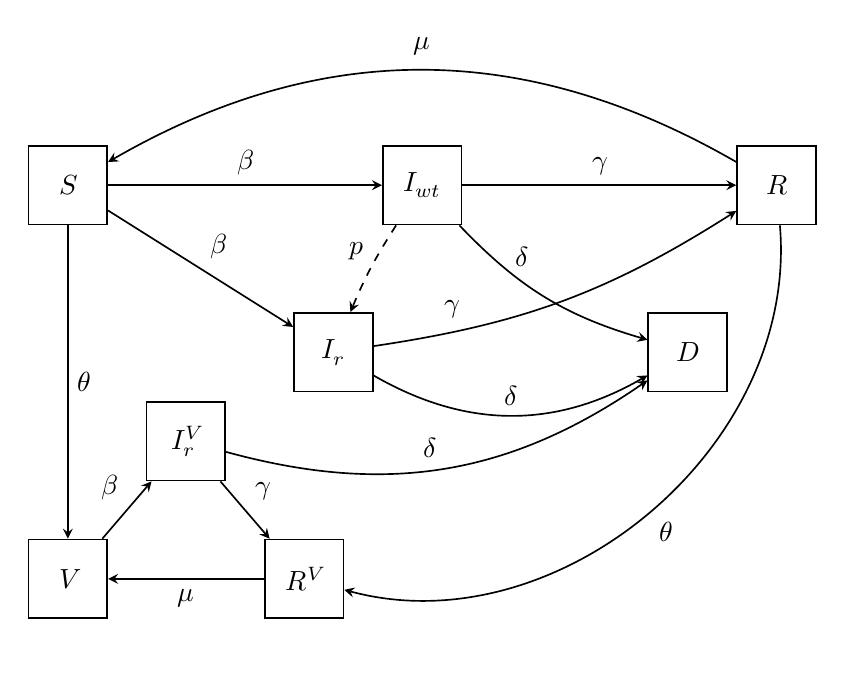
\begin{tikzpicture}[>= stealth, shorten >= 0pt,
                    auto, node distance=4.5cm, semithick]
\tikzstyle{every state}=[shape=rectangle, draw=black, 
                    semithick, inner sep=1pt, minimum size=1cm]
  \node[state] (S) {$S$};
  \node[state] (Iwt) [right of=S] {$I_{wt}$};
  \node[state] (R)   [right of=Iwt] {$R$};
  \node[state] (Ir)  [below right of=S, node distance=3cm, xshift=1.25cm] {$I_r$};
  \node[state] (D)   [right of=Ir] {$D$};
  \node[state] (V)   [below of=S, node distance=5cm] {$V$};
  \node[state] (IrV) [above right of=V, node distance=2.12cm, yshift=0.25cm] {$I_r^V$};
  \node[state] (RV)  [right of=V, node distance=3cm] {$R^V$};
  \path[->]    (S)   edge node {$\beta$} (Iwt);
  \path[->]    (S)   edge node {$\theta$} (V);
  \path[->]    (Iwt) edge node {$\gamma$} (R);
  \path[->]    (R)   edge [bend right=30] node [yshift=0.55cm] {$\mu$} (S);
  \path[->]    (Iwt) edge [bend right=15] node [yshift=0.25cm,xshift=-0.5cm] {$\delta$} (D);
  \path[->]    (R)   edge [bend left=55] node {$\theta$} (RV);
  \path[->]    (RV)  edge node {$\mu$} (V);
  \path[->]    (V)   edge node {$\beta$} (IrV);
  \path[->]    (IrV) edge node {$\gamma$} (RV);
  \path[->]    (IrV) edge [bend right=25] node {$\delta$} (D);
  \path[->]    (S)   edge node {$\beta$} (Ir);
  \path[->]    (Ir)  edge [bend right=12] node [yshift=-0.35cm, xshift=-1.2cm] {$\gamma$} (R);
  \path[->]    (Ir)  edge [bend right=30] node {$\delta$} (D);
  \path[->]    (Iwt) edge [style=dashed, bend right=5] node [yshift=0.45cm, xshift=-0.4cm] {$p$} (Ir);
\end{tikzpicture}
\end{center}
\end{figure}

\begin{figure}[H]
\caption{Compartmental model of Rella et alia (2021), extended to allow vaccinated individuals to return to being susceptible.}
\begin{center}
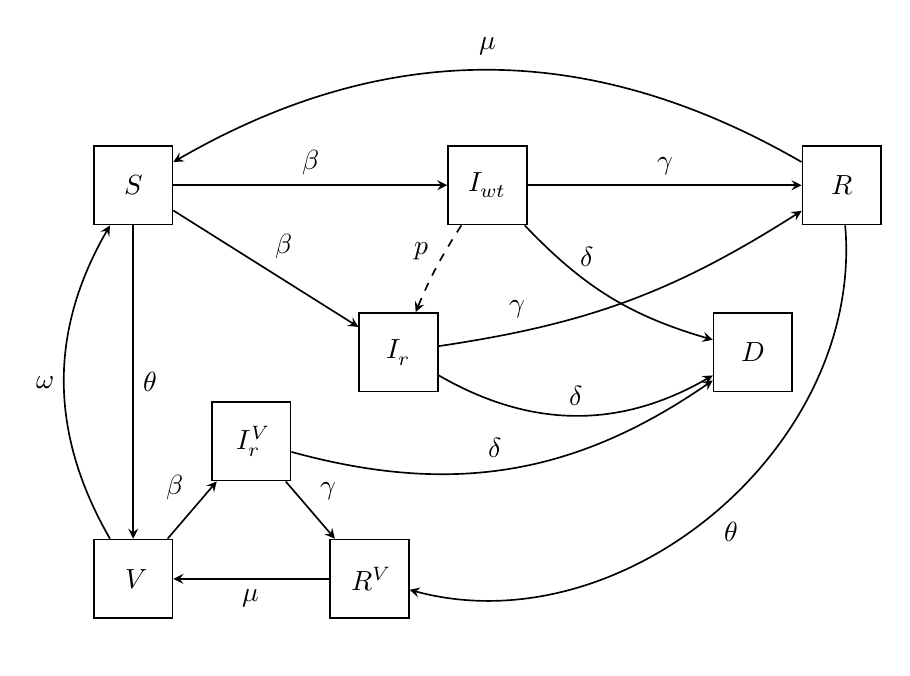
\begin{tikzpicture}[>= stealth, shorten >= 0pt,
                    auto, node distance=4.5cm, semithick]
\tikzstyle{every state}=[shape=rectangle, draw=black, 
                    semithick, inner sep=1pt, minimum size=1cm]
  \node[state] (S) {$S$};
  \node[state] (Iwt) [right of=S] {$I_{wt}$};
  \node[state] (R)   [right of=Iwt] {$R$};
  \node[state] (Ir)  [below right of=S, node distance=3cm, xshift=1.25cm] {$I_r$};
  \node[state] (D)   [right of=Ir] {$D$};
  \node[state] (V)   [below of=S, node distance=5cm] {$V$};
  \node[state] (IrV) [above right of=V, node distance=2.12cm, yshift=0.25cm] {$I_r^V$};
  \node[state] (RV)  [right of=V, node distance=3cm] {$R^V$};
  \path[->]    (S)   edge node {$\beta$} (Iwt);
  \path[->]    (S)   edge node {$\theta$} (V);
  \path[->]    (Iwt) edge node {$\gamma$} (R);
  \path[->]    (R)   edge [bend right=30] node [yshift=0.55cm] {$\mu$} (S);
  \path[->]    (Iwt) edge [bend right=15] node [yshift=0.25cm,xshift=-0.5cm] {$\delta$} (D);
  \path[->]    (R)   edge [bend left=55] node {$\theta$} (RV);
  \path[->]    (RV)  edge node {$\mu$} (V);
  \path[->]    (V)   edge node {$\beta$} (IrV);
  \path[->]    (IrV) edge node {$\gamma$} (RV);
  \path[->]    (IrV) edge [bend right=25] node {$\delta$} (D);
  \path[->]    (S)   edge node {$\beta$} (Ir);
  \path[->]    (Ir)  edge [bend right=12] node [yshift=-0.35cm, xshift=-1.2cm] {$\gamma$} (R);
  \path[->]    (Ir)  edge [bend right=30] node {$\delta$} (D);
  \path[->]    (Iwt) edge [style=dashed, bend right=5] node [yshift=0.45cm, xshift=-0.4cm] {$p$} (Ir);
  \path[->]    (V) edge [bend left=30] node {$\omega$} (S);
\end{tikzpicture}
\end{center}
\end{figure}

\begin{figure}[H]
\caption{Compartmental model for capturing waning immunity and incomplete vaccination.}
\begin{center}
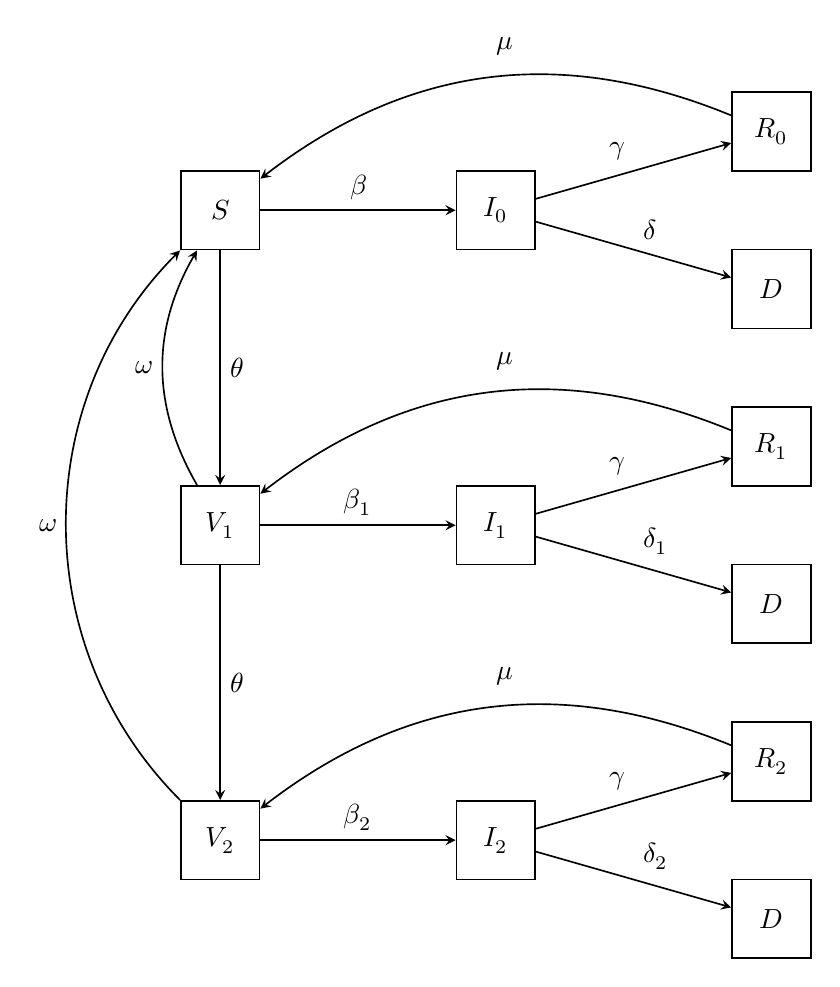
\begin{tikzpicture}[>= stealth, shorten >= 0pt,
                    auto, node distance=3.5cm, semithick]
\tikzstyle{every state}=[shape=rectangle, draw=black, 
                    semithick, inner sep=1pt, minimum size=1cm]
  \node[state] (S) {$S$};
  \node[state] (I0) [right of=S] {$I_0$};
  \node[state] (R0) [right of=I0, yshift=1cm] {$R_0$};
  \node[state] (D0)  [right of=I0, yshift=-1cm] {$D$};
  %
  \node[state] (V1) [below of=S, node distance=4cm] {$V_1$};
  \node[state] (I1) [right of=V1] {$I_1$};
  \node[state] (R1) [right of=I1, yshift=1cm] {$R_1$};
  \node[state] (D1) [right of=I1, yshift=-1cm] {$D$};
  %
  \node[state] (V2) [below of=V1, node distance=4cm] {$V_2$};
  \node[state] (I2) [right of=V2] {$I_2$};
  \node[state] (R2) [right of=I2, yshift=1cm] {$R_2$};
  \node[state] (D2) [right of=I2, yshift=-1cm] {$D$};
  %
  \path[->]  (S)  edge node {$\beta$} (I0);
  \path[->]  (V1) edge node {$\beta_1$} (I1);
  \path[->]  (V2) edge node {$\beta_2$} (I2);
  \path[->]  (S)  edge node {$\theta$} (V1);
  \path[->]  (V1) edge node {$\theta$} (V2);
  \path[->]  (V1) edge [bend left=30] node {$\omega$} (S);
  \path[->]  (V2) edge [bend left=45] node {$\omega$} (S);
  %
  \path[->]  (I0) edge node {$\gamma$} (R0);
  \path[->]  (I1) edge node {$\gamma$} (R1);
  \path[->]  (I2) edge node {$\gamma$} (R2);
  %
  \path[->]  (R0) edge [bend right=30] node [yshift=0.65cm] {$\mu$} (S);
  \path[->]  (R1) edge [bend right=30] node [yshift=0.65cm] {$\mu$} (V1);
  \path[->]  (R2) edge [bend right=30] node [yshift=0.65cm] {$\mu$} (V2);
  %
  \path[->]  (I0) edge node {$\delta$} (D0);
  \path[->]  (I1) edge node {$\delta_1$} (D1);
  \path[->]  (I2) edge node {$\delta_2$} (D2);
\end{tikzpicture}
\end{center}
\end{figure}



\end{document}
